\chapter{Conclusion}
In the future, ubiquitous sensors will constantly monitor your health and assess your risk for life threatening conditions.  Many life threatening conditions can be cured if treated early enough.  Further, many life threatening conditions are obvious to a trained medical expert.  The recent advances in AI can be leveraged to distill some of this highly valuable medical expertise.  Consequently, it can be distributed widely, run all the time, and cost little more than the cost of electricity that runs it.  In this thesis I argued that future is not so distant.  Specifically I showed results in detecting skin cancer from photos that any smartphone can take, and assessing risk for a wide range of heart and other internal organ conditions from waveform signals such as ECG and PPG, both of which a smartwatch can measure.

\section{Dermatology}
As researchers and clinicians delve into the medical applications of artificial intelligence (AI) and develop deep learning-based tools, dermatology's visually oriented tasks stand out as ripe for innovation. Both providers and patients have ready access to the tissue of interest, and with their smartphones, they possess the imaging devices needed to collect data at scale. There have been a number of recent advances on automated skin lesion classification tools. The dermatological applications of AI hold both opportunities and pitfalls as they cross from pixels to practice, deploying these tools across diverse patient populations.

\subsection{Contextual learning in lesion classification}
A robust AI system of automated solitary lesion classification may be feasible for clinical integration and can augment clinical practice. However, the greatest utility would come from a one-system contextual learning model for multiple tasks that accommodates multimodal input, detection of changes in lesions, and comparison of lesions to others on the body. Without multi-lesion change detection and classification capability, consumer-facing technology runs the risk of reassuring a hypothetical patient about the lentigo on her arm, while missing the melanoma on her leg. Lesion classification can also benefit from multimodal inputs such as age, gender, race, location on the body, or examples of other lesions on the body.

A one-system model may be capable of answering a number of clinical questions across a breadth of dermatological diseases, beyond the binary classification of benign versus malignant \cite{kuprel2017dermatologist}, whereas from a logistical and usability perspective, it may be suboptimal to have a different model for each skin type or clinical classification task. Multiple models may worsen the performance of the algorithm on “edge” cases, such as patients with intermediate skin types or background skin disease (i.e., a patient with extensive psoriasis and squamous cell carcinoma). Furthermore, a task-specific classifier may fall short if mistakes are made in selecting the initial task. An AI model for dermatology that generalizes between multiple tasks and transfers abilities to new tasks using prior experience with similar tasks would also be the most clinically functional and streamlined solution. Although there may be fewer data for some skin types, the benefits of training a joint model with sufficient data may outweigh its limitations.

\subsection{Nonstandardized and standardized input in AI classification}
Making an artificially intelligent system robust enough to handle the variation inherent in image input also poses a hurdle, yet supports the technology’s potential for scalability. Dermatology images are the easiest to capture of all medical images, but also the least standardized. Standardization of images is difficult, even with dermoscopic images. Variability must be incorporated into training algorithms to create capacity to handle noisy data. This includes multiple camera angles, different orientations, blurry photos, multiple skin backgrounds, pen markings or rulers included in the photo, or variations in lighting. Otherwise, the algorithm will use features of nonstandardized photos to guide decision making. For instance, the net appeared more likely to interpret images with rulers as malignant. Why? In the dataset, images with rulers were more likely to be malignant; thus the net inadvertently learned that rulers are malignant. These biases in AI models are inherent unless specific attention is paid to address inputs with variability.  An alternative approach is to incorporate stringent standards and/or hardware that allows for standardization of photos, at the cost of decreased potential for scalability.

Unanswered questions remain with wide-open image collection: (1) How can safe limits be defined the for analysis given the input — for example, how can one determine whether a blurry image or dark image is too dark or too blurry? (2) Can the issue of fidelity be addressed, whereby analysis of images of the same lesion, for example, rotated or oriented differently, or with different angle, zoom, or brightness, outputs a stable result? One example of a hybrid intermediate approach might be to incorporate an initial algorithm that determines the suitability of an image for analysis, much as modern banking smartphone apps detect the presence of a check in a picture before depositing it.

\subsection{Models with robust training and clinical validation}
When incorporating AI tools in the clinic, they should aim to eliminate biases with inclusion of training images and data from a breadth of practice and patients. Subsequent prospective clinical validation demonstrating the robustness of a tool to handle the variability inherent in data input and diversity of patient population is necessary before public adoption for a role in medical decision augmentation. Without this stringency, there exists the potential for unintended effects and inherent bias to exist within these tools. When assessing the clinical relevance and validity of an algorithm, area under the curve is a valid metric for validating clinical performance of binary classifiers. Area under the curve reports across every threshold and every prevalence. The net was trained to answer any number of clinical questions because it was trained across the breadth of dermatological disease rather than just training on a certain number of diagnoses, so multiple areas under the curve were able to tell how the tool would perform if a user were to freely input a skin lesion.

One of the complexities of AI research in a connected world is balancing the risks and benefits of making publicly available an algorithm that has not been validated prospectively. A publicly available algorithm engages a broader community, allowing for rapid assessment and evaluation of both its capacity to handle varied data and its biases. The posited risk lies in creating the potential for an AI tool to reach or be inappropriately wielded by or for an individual who may be falsely reassured, alarmed, or otherwise use the tool in an unintended manner. Disclaimers regarding the investigative nature of a tool certainly are one approach and may satisfy some as sufficient. Another option is granting exclusive access to researchers and clinicians for a certain period before a tool is released to the general public. Such an approach may help balance the rich and fruitful discussion that comes from open-source engagement with such a tool with the safety of the public.

Use of deep neural networks in the classification of skin lesions has made rapid progress in recent years while simultaneously generating significant hype. As researchers continue improving on these models and building high-quality databases with increased data input modalities, they must continue addressing the many nuances involved in bringing these new technologies safely to the bedside.

\section{Critical Care}

The goal was to determine what information, if any, could be obtained from biological waveforms such as ECG and PPG.  The answer is that a lot of information, actually, can be determined from biological waveforms.  First it was shown that relative risk can be assessed.  That is, what is the user's risk relative to what the prevalence of a condition is?  It was shown that users could be reliably placed into various risk groups.  Second, it was shown that on a population level, users could be triaged with a cheap, ubiquitous, but maybe unreliable test to take a more expensive, limited, but reliable test.  When using the neural net to triage, this resulted in a significant proportion of sick users detected.  One could imagine a smartwatch sending users a notification to get an MRI or biopsy, for example.  Finally it was shown that the neural net had a general sense of the organs in the body based on the biological waveforms it was trained on.  That is, brain conditions were nearby in a semantic space, liver conditions were close to one another, heart conditions formed a cluster, and so on.  One could imagine a semantic heat map like this tracking users' organ health based on data collected from their smartwatch.

\section{Future}

\begin{figure}
\begin{center}
    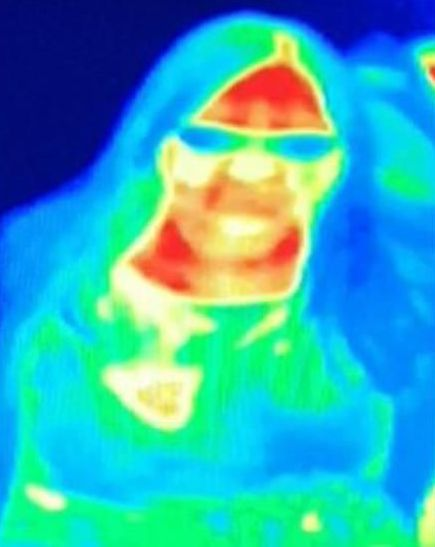
\includegraphics[width=0.25\textwidth]{intro_breast_cancer}
\end{center}
\caption{Thermal Camera Detects Breast Cancer}
\vspace{12px}
Bal Gill, 41, of Berkshire, England, had stopped by Camera Obscura \& World of Illusions in Edinburgh, Scotland, during a family vacation. When she went into the museum's thermal imaging camera room she noticed her left breast was a different color. When she returned home she saw a doctor who confirmed she had breast cancer.
\vspace{12px}
\label{fig:intro_breast_cancer}
\end{figure}

For a long time medicine has focused on helping the sick.  This is a noble endeavor, but maybe we can do better.  Maybe we can prevent people from getting sick in the first place.  They say that an ounce of prevention is worth a pound of cure.  We are constantly surrounded by advanced technology.  The intersection of preventive health and AI is highly fertile ground, for example

\begin{itemize}
    \item When you go through the airport an expensive scanner sends harmless millimeter waves through your body to determine if you are carrying something dangerous.  But while they are at it, why not do a quick check for tumors too?
    \item People are often taking high resolution photos with friends with modern smartphone cameras.  Maybe these photos could be processed for skin cancer in the background.
    \item A great deal of information is contained in stool and urine.  Maybe a smart toilet could analyze it.
    \item Over 100 million people wear smartwatches that are capable of measuring electrocardiograms and photoplethysmograms.  From an ECG alone, atrial fibrillation can be detected.  Maybe other conditions can be detected from these smartwatches.
    \item When a woman went into a museum's thermal imaging camera room she noticed her left breast was a different colour \ref{fig:intro_breast_cancer}. When she returned home she saw a doctor who confirmed she had breast cancer.  AI could automate this detection.
    \item Television viewers have detected thyroid cancer on reporters by noticing a lump on the neck.  Maybe AI could automate this detection in all videos posted to the internet.
\end{itemize}

A semantic map as shown in Chapter 3 Figure \ref{fig:icu_icd_map} can be formed for all medical conditions.  A personal heat map can then be updated with every new piece of health data gathered about the user, lighting up the regions where the user is healthy or unhealthy.  For example if they are experiencing heart problems, the region of the semantic map related to heart conditions will light up red.  If they exercise a lot and have a healthy heart, that region will light up green.  The data gathered on the user could include biological waveforms, images of skin lesions, data from a smart toilet, data from a smart bathtub, data from airport scanners, selfies in your camera roll, public videos of you on the internet, data from ubiquitous sensors everywhere.  When a user begins to deviate from healthy, AI will detect it long before any traditional symptoms are present.  In control theory there is a dynamical system (e.g. human body), and a desired target (e.g. healthy). I predict that in the near future we will use ubiquitous sensors and AI to observe the human body more deeply and more frequently, allowing users to correct small perturbations and maintain health.  An ounce of prevention is worth a pound of cure.